% Fig 6:fig3 -- Esquema del grafo de conocimiento electoral (10 nodos / 7 relaciones).
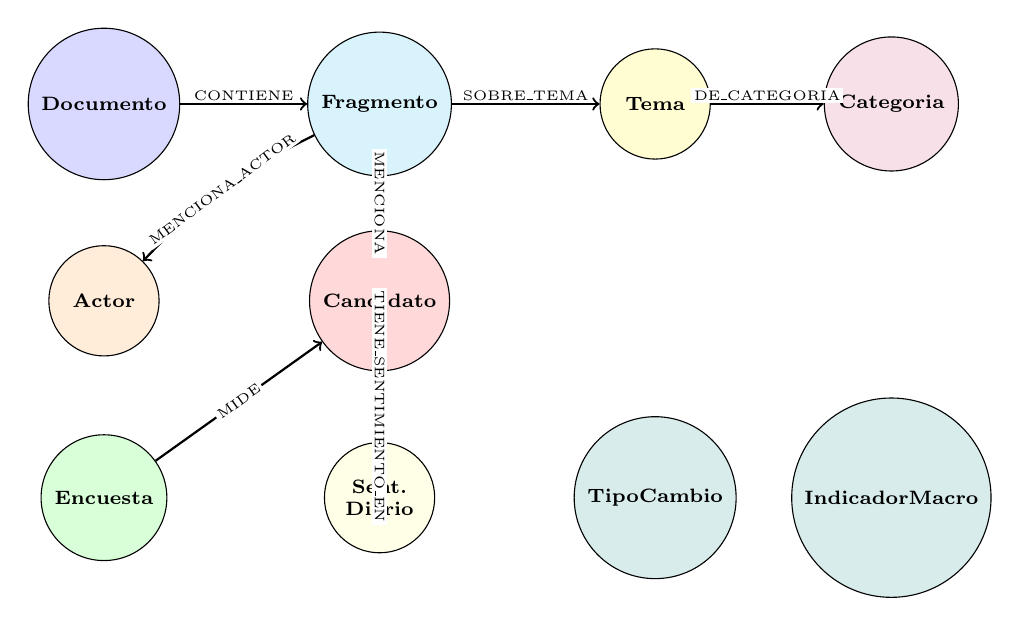
\begin{tikzpicture}[
    node distance=0.6cm,
    every node/.style={font=\scriptsize, align=center, inner sep=4pt},
    nodo/.style={draw, circle, minimum size=1.4cm, font=\scriptsize\bfseries},
    doc/.style={nodo, fill=blue!15},
    frag/.style={nodo, fill=cyan!15},
    tema/.style={nodo, fill=yellow!18},
    actor/.style={nodo, fill=orange!15},
    cand/.style={nodo, fill=red!15},
    cat/.style={nodo, fill=purple!12},
    enc/.style={nodo, fill=green!15},
    macro/.style={nodo, fill=teal!15},
    rel/.style={font=\tiny, fill=white, inner sep=1pt}
]
    \node[doc]   (doc)   at (0, 2)      {Documento};
    \node[frag]  (frag)  at (3.5, 2)    {Fragmento};
    \node[tema]  (tema)  at (7, 2)      {Tema};
    \node[cat]   (cat)   at (10, 2)     {Categoria};

    \node[cand]  (cand)  at (3.5, -0.5) {Candidato};
    \node[actor] (actor) at (0, -0.5)   {Actor};

    \node[enc]   (enc)   at (0, -3)     {Encuesta};
    \node[nodo, fill=yellow!10] (sd) at (3.5, -3) {Sent.\\Diario};
    \node[macro] (tc)    at (7, -3)     {TipoCambio};
    \node[macro] (im)    at (10, -3)    {IndicadorMacro};

    % Relaciones
    \draw[->, thick] (doc) -- node[rel, above] {CONTIENE} (frag);
    \draw[->, thick] (frag) -- node[rel, above] {SOBRE\_TEMA} (tema);
    \draw[->, thick] (tema) -- node[rel, above] {DE\_CATEGORIA} (cat);
    \draw[->, thick] (frag) -- node[rel, sloped] {MENCIONA} (cand);
    \draw[->, thick] (frag) to[bend right=10] node[rel, sloped] {MENCIONA\_ACTOR} (actor);
    \draw[->, thick] (enc)  -- node[rel, sloped] {MIDE} (cand);
    \draw[->, thick] (cand) -- node[rel, sloped] {TIENE\_SENTIMIENTO\_EN} (sd);
\end{tikzpicture}
